
%(BEGIN_QUESTION)
% Copyright 2015, Tony R. Kuphaldt, released under the Creative Commons Attribution License (v 1.0)
% This means you may do almost anything with this work of mine, so long as you give me proper credit

En nyttig strategi for kvalitativ analyse av reguleringsstrategier er å merke inngangene til flerinngangsfunksjoner med ``+'' eller ``$-$'' for å vise virkningsretning. Dette er samme symbolikk som brukes for inngangene på en operasjonsforsterker, der ``+'' er ikke-inverterende inngang og ``$-$'' er inverterende inngang. Man kan faktisk se på en operasjonsforsterker som en proporsjonalregulator med svært høy forsterkning ($k$):

$$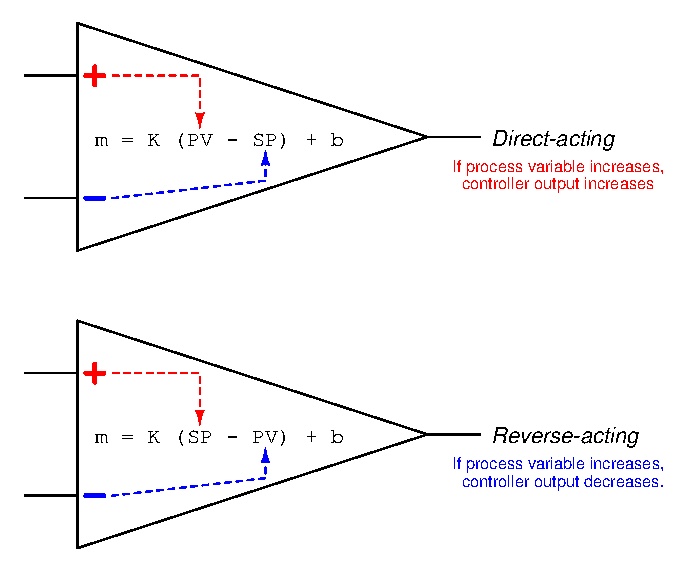
\includegraphics[width=15.5cm]{i01171x01.eps}$$

For å illustrere dette konseptet, se på disse to diagrammene av et enkeltsløyfe-reguleringssystem. I diagrammet til venstre er regulatoren vist med standard ISA-symbolikk. I skissen til høyre er regulatoren vist med opamp-symbolikk i stedet. I begge tilfeller må regulatoren være {\it reversvirkende} for å stabilisere prosessen, men ``+''- og ``$-$''-symbolene gjør det enklere å skille virkningsretning for prosessvariabelen kontra settpunktet:

$$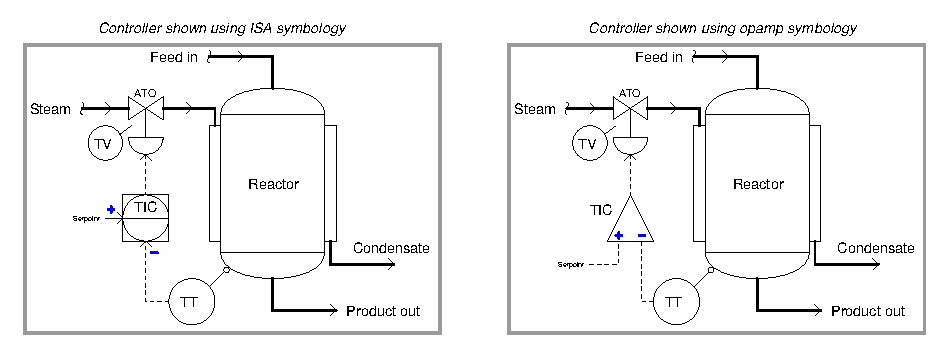
\includegraphics[width=15.5cm]{i01171x02.eps}$$

\filbreak

Tegn inn egne ``+''- og ``$-$''-merkinger ved inngang(ene) til hver regulator i disse strategidiagrammene, slik at riktig virkningsretning vises for at hvert system skal fungere korrekt. For å hjelpe deg med dette bruker høyre versjon av hvert diagram opamp-symbolikk for regulatoren i stedet for ISA-symbolikk. Anta direktevirkende transmittere i alle tilfeller, og vær spesielt oppmerksom på virkningsretningen til hver reguleringsventil:

$$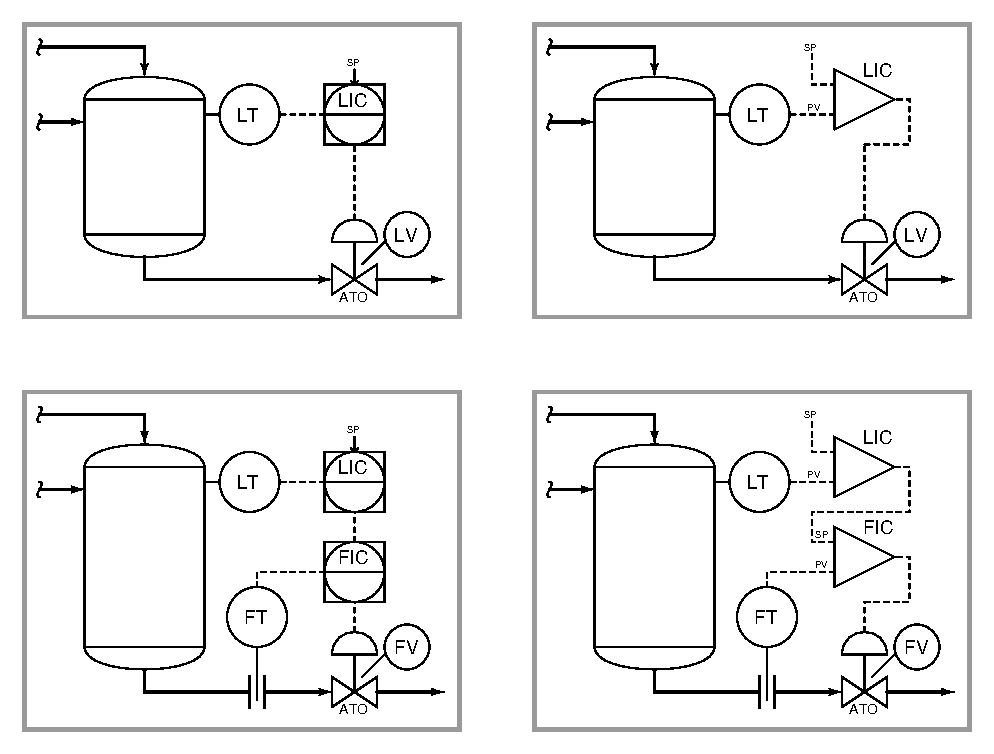
\includegraphics[width=15.5cm]{i01171x03.eps}$$

\vskip 20pt \vbox{\hrule \hbox{\strut \vrule{} {\bf Forslag til sokratisk diskusjon} \vrule} \hrule}

\begin{itemize}
\item{} Gjør en serie ``tankeeksperimenter'' der du ser for deg at prosessvariabelen endrer verdi på grunn av endret prosesslast, og analyser deretter hvordan hver regulator reagerer i hvert system. Hvordan hjelper ``+''- og ``$-$''-merkingen analysen din?
\item{} Hva legger du merke til ved virkemåten til master- og slaveregulatorene i kaskadesystemene, og hvordan disse må være for ATO kontra ATC-ventiler? Overrasker dette resultatet deg?
\item{} Forklar hvorfor det bare gir mening å merke {\it inngangene} til en regulator med ``polaritet''-symboler og ikke {\it utgangen} fra regulatoren.
\end{itemize}

\underbar{file i01171}
%(END_QUESTION)





%(BEGIN_ANSWER)

$$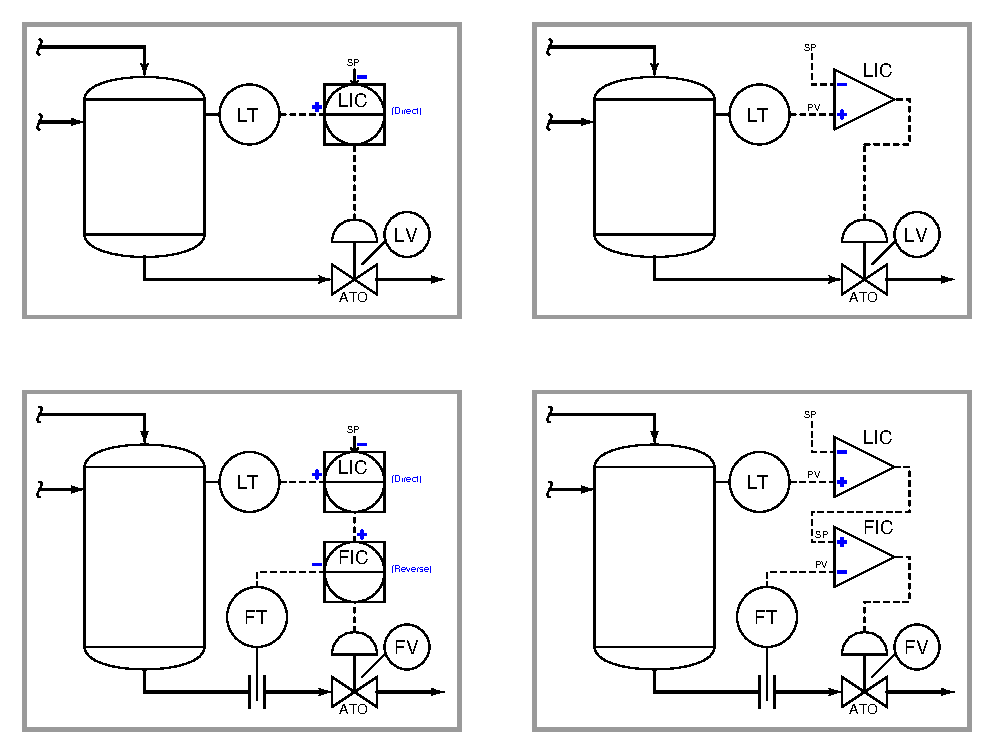
\includegraphics[width=15.5cm]{i01171x04.eps}$$

Merk at ordene ``direkte'' og ``revers'' er overflødige når ``+''- og ``$-$''-merking brukes. En regulator med ``+'' ved PV-inngangen er per definisjon direktevirkende; en regulator med ``$-$'' ved PV-inngangen er per definisjon reversvirkende.
 
%(END_ANSWER)





%(BEGIN_NOTES)

Her vises nødvendig regulatorvirkemåte dersom reguleringsventilen er Air-To-Close (ATC) i stedet for Air-To-Open (ATO):

$$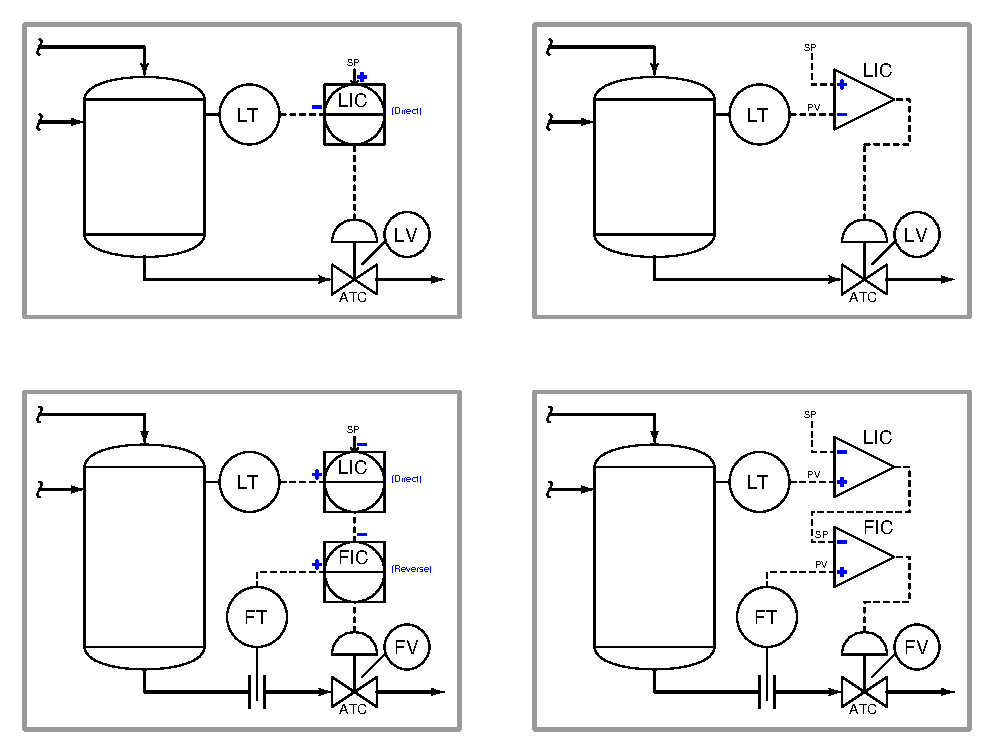
\includegraphics[width=15.5cm]{i01171x05.eps}$$


%INDEX% Grunnleggende regulering: direkte versus revers regulatorvirkning
%INDEX% Regulering, strategier: kaskadert regulatorvirkning

%(END_NOTES)
